\section{Heat exchangers}
\quad\, The last important component that has to be defined and characterized is the heat-exchanger (HX). As the name says, the purpose of this element is to transfer the heat from a \textbf{hot} fluid to a \textbf{cold} fluid. The heat-exchangers can be classified into several categories\citep{Ngendakumana2018}.

\begin{itemize}
\setstretch{1}
\item The recuperators: their purpose is to recover the heat from a hot fluid to heat up a cold fluid for direct usage. For instance, the exhaust gas from a boiler will go through a recuperator to exchange its energy with water. For this application and for many others, the two streams within the HX are separated by physical walls.

Alternatively, the heat exchange can be performance by direct contact between the two fluids. In this case, nothing prevents the hot flow to mix with the cold flow (and vice versa).
\item The regenerators: considering a cycle , the purpose of the regenerators is to use a hot flow from the cycle to heat up a cold flow from the same cycle. 
\end{itemize}

By definition, the hot stream is the one that \textbf{provides} the heat, and the cold stream is the one \textbf{receiving} the heat.

On the Figure \ref{fig:C3_HX} are illustrated some schematics of heat-exchanger owning at different families.
\begin{figure}[h]
\centering
\subfloat[HX with fined plates \citep{Ngendakumana2018}\label{fig:C3_HX_fin_plate}]{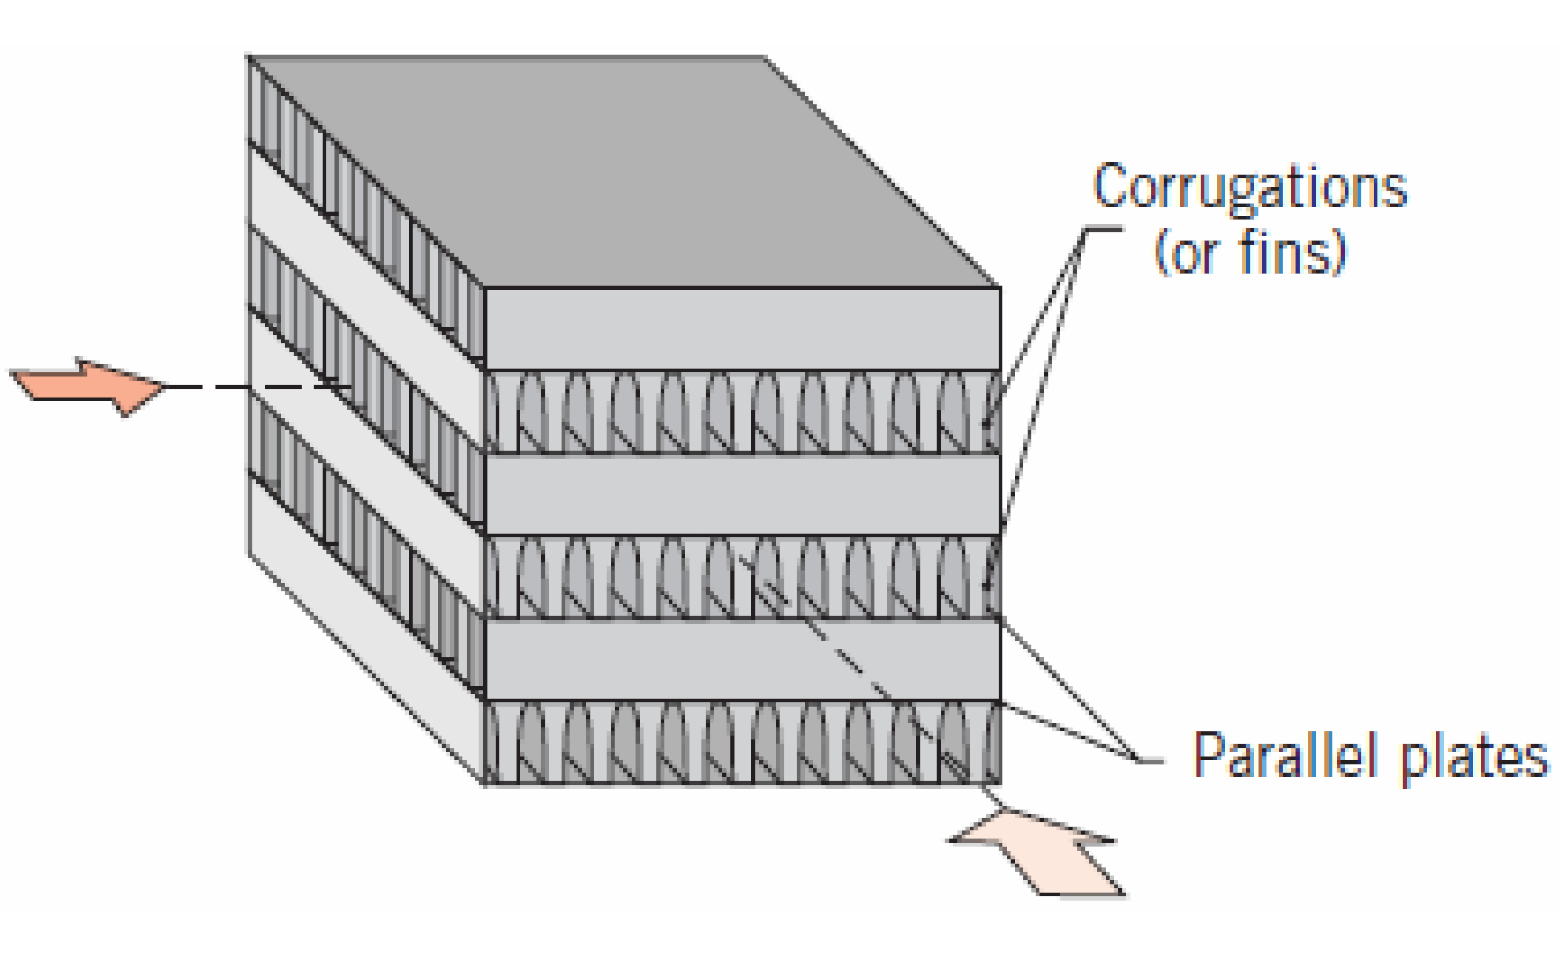
\includegraphics[width=0.4\textwidth]{HX_fin_plate}}\hfill
\subfloat[HX with fined tubes \citep{Ngendakumana2018}\label{fig:C3_HX_fin_tube}] {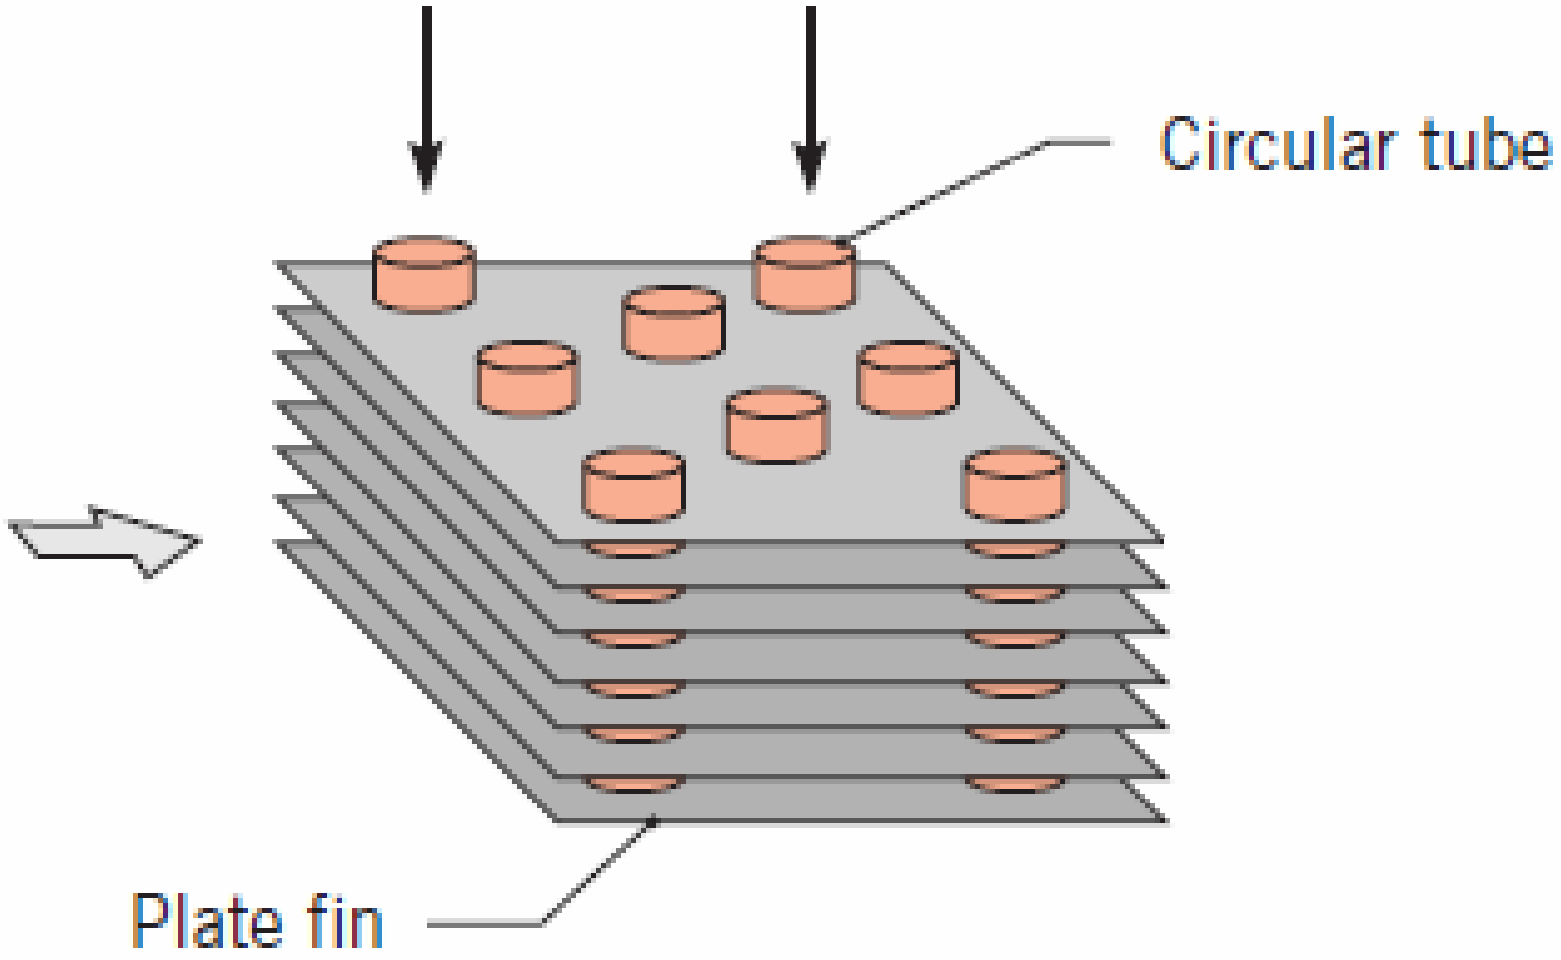
\includegraphics[width=0.4\textwidth]{HX_fin_tube}}\hfill
\subfloat[Plate heat exchangers \citep{Ngendakumana2018}\label{fig:C3_PHE}]{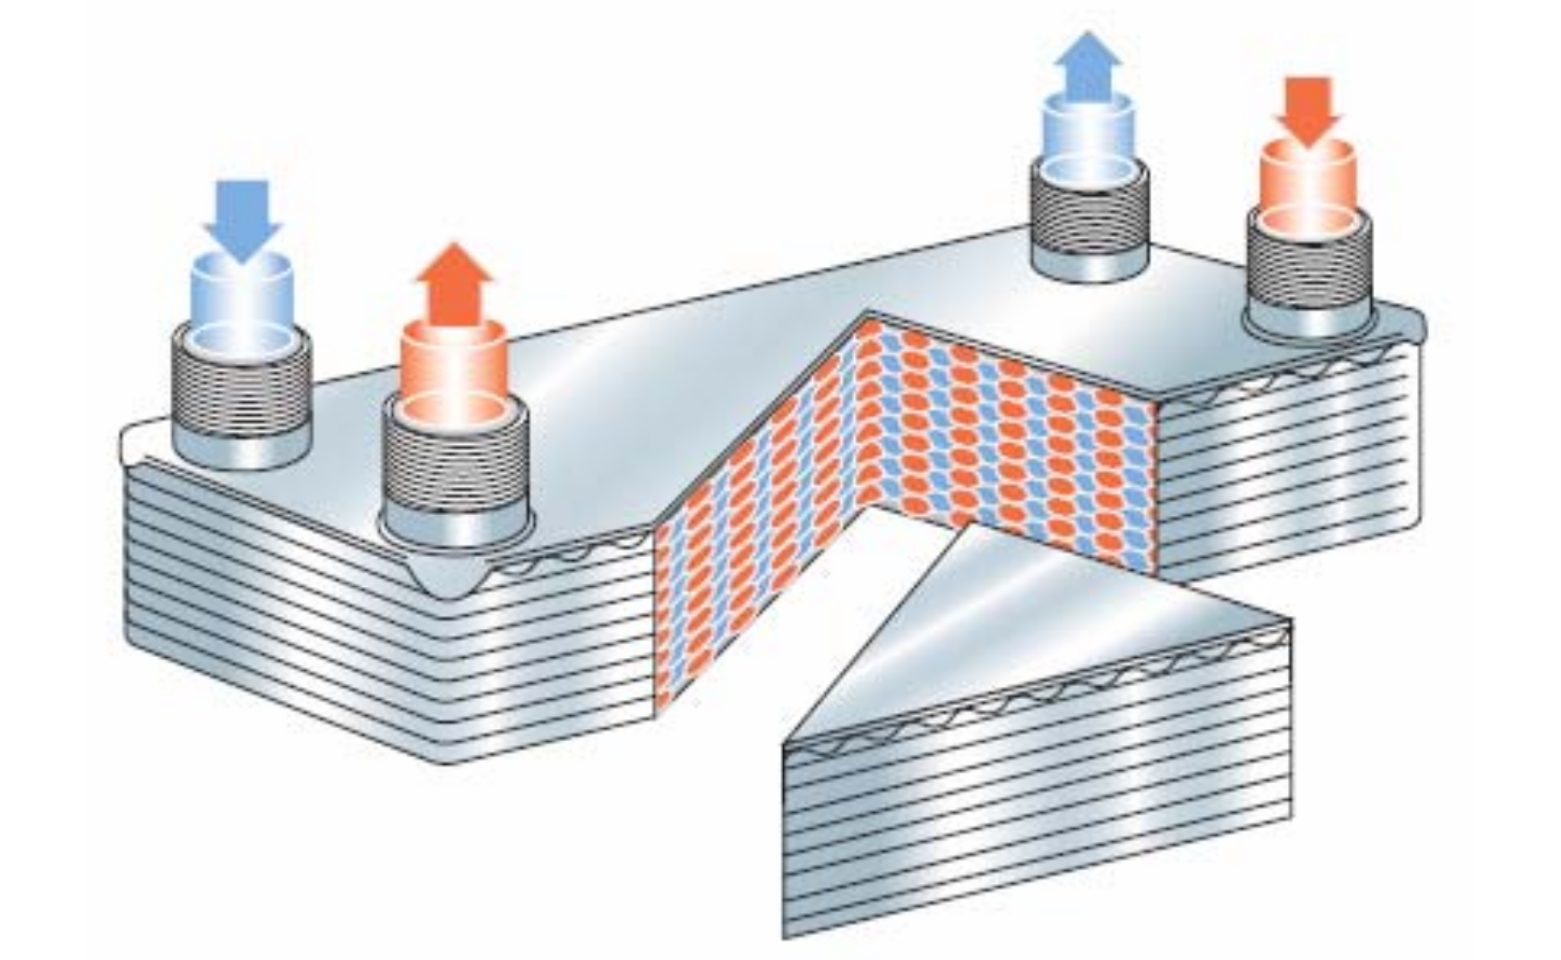
\includegraphics[width=0.4\textwidth]{HX_brased_plate}}
\caption{HX illustrations} \label{fig:C3_HX}
\end{figure}

The selected family will highly depends on the type of application that is targeted. Plate heat exchangers are one of the most compact type of heat exchangers. This compactness is highly appreciated for any system where the foot print and volume has to be as minimal as possible. However, this is at the cost of more complicated maintenance due the brazing of the plates.

This section will not cover the specificity of these different families. Instead, the main notions which are necessary to characterized the heat transfer between two fluids will be given.

\subsection{Stream configurations}
\quad\, There isn't an unique configuration regarding about the interaction between the hot and cold streams. Indeed, here are the main categories based on flow configurations.

\begin{itemize}
\setstretch{1}
\begin{figure}[h]
\centering
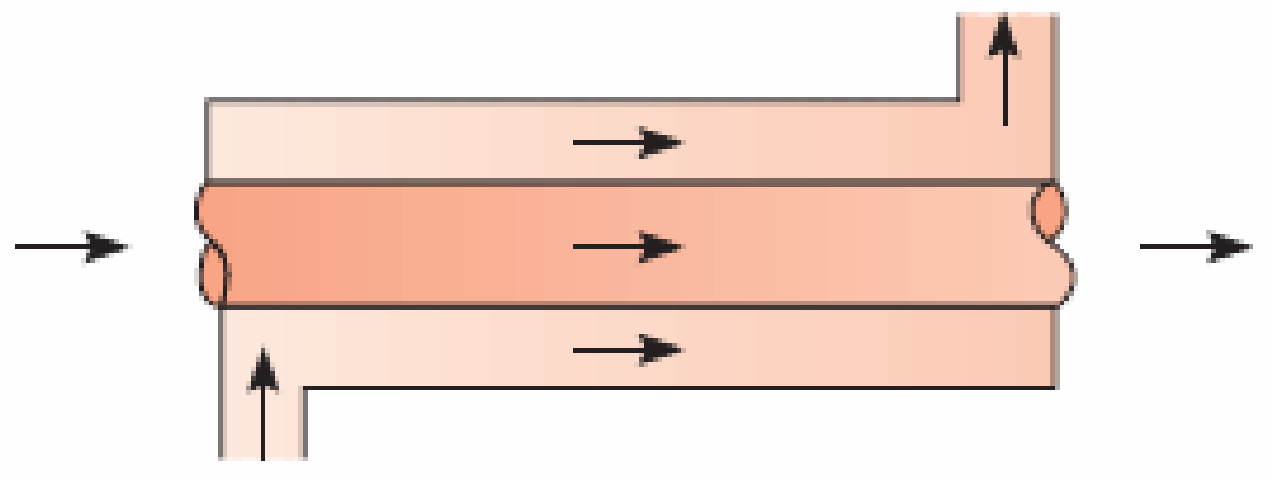
\includegraphics[width=0.4\textwidth]{parallele_flow}
\caption{Parallel flow heat exchanger \citep{Ngendakumana2018}}
\label{fig:C3_para_flow}
\end{figure}

\item Parallel flow HX: The two streams go through the heat exchanger in the same direction. 

\begin{figure}[h]
\centering
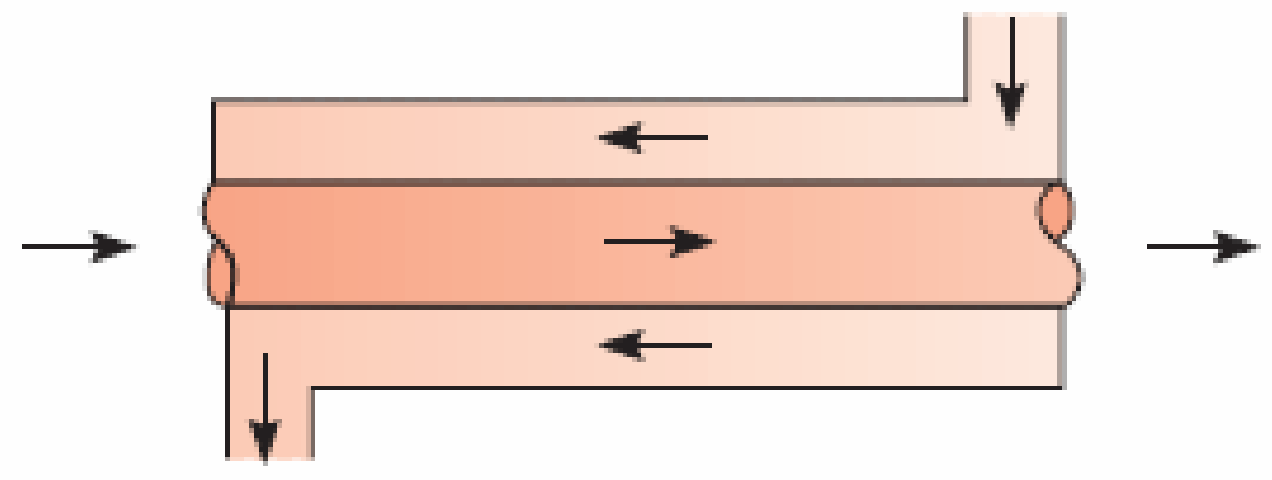
\includegraphics[width=0.4\textwidth]{opposite_flow}
\caption{Counter flow heat exchanger \citep{Ngendakumana2018}}
\label{fig:C3_counter_flow}
\end{figure}

\item Counter flow HX: The two streams go through the heat exchanger in the opposite direction. This configuration is more frequent than the parallel flow HX due to higher efficiency.

\begin{figure}[h]
\centering
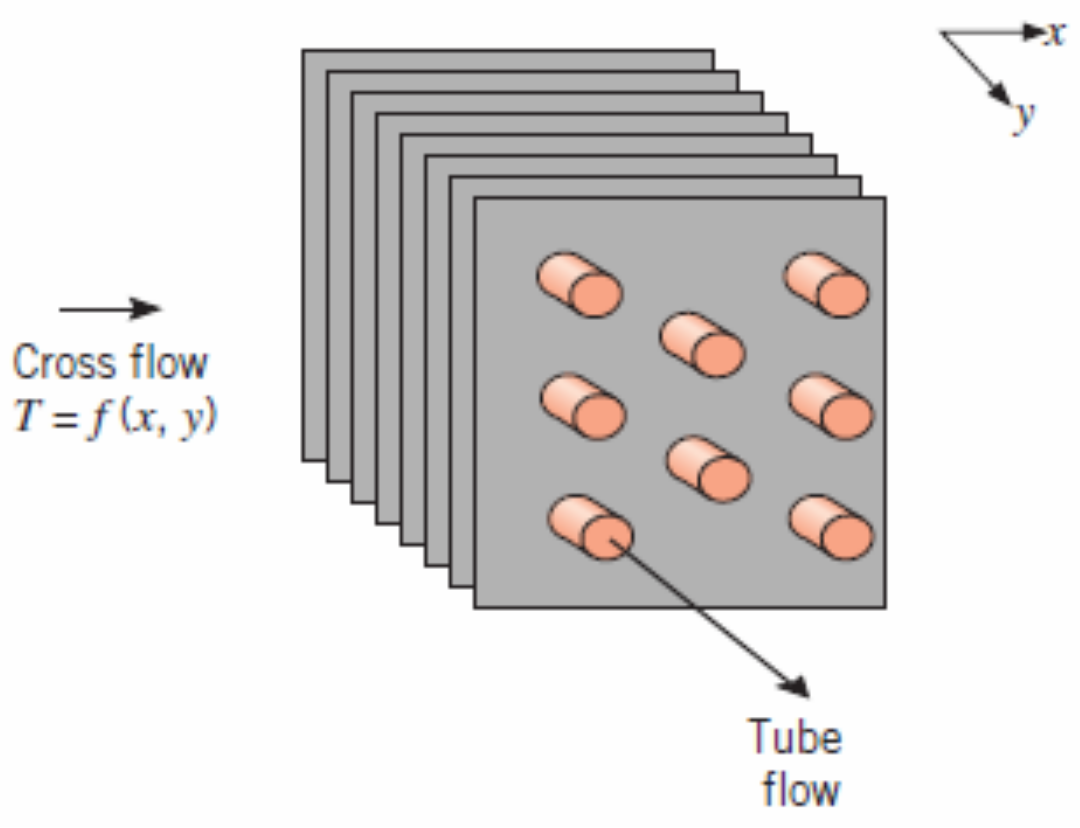
\includegraphics[width=0.4\textwidth]{crossed_flow_non_mixed}
\caption{Cross flow heat exchanger, both fluids unmixed \citep{Ngendakumana2018}}
\label{fig:C3_cross_flow_unmixed}
\end{figure}

\item Cross flow HX, both fluids unmixed: The flow in the tube does not sees the property of cross flow varying along with the distance traveled. Both flow are unmixed.
\newpage
\begin{figure}[h]
\centering
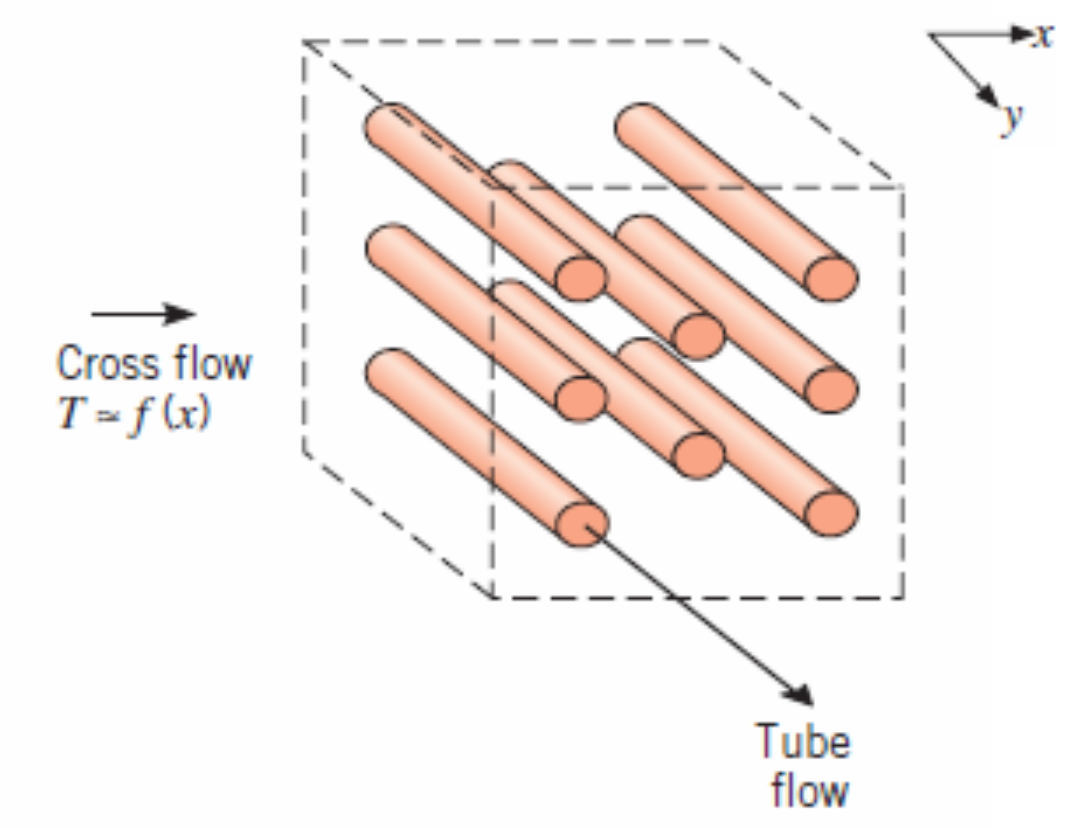
\includegraphics[width=0.4\textwidth]{crossed_flow_one_mixed}
\caption{Cross flow heat exchanger, one fluid mixed \citep{Ngendakumana2018}}
\label{fig:C3_cross_flow_1mixed}
\end{figure}

\item Cross flow HX, one fluid mixed: The flow in the tube does not sees the property of cross flow varying along with the distance traveled. The cross flow does not travel inside isolated channels.
\end{itemize}

Considering the parallel and counter flow heat exchanger, Two temperature differences can be defined based on the temperature profiles (Figure \ref{fig:C3_Tprof}) of both fluids inside the heat exchanger.

\begin{figure}[h]
\centering
\subfloat[Temperature profil for parallel flow HX \citep{Ngendakumana2018}\label{fig:C3_HX_par_flow_T}]{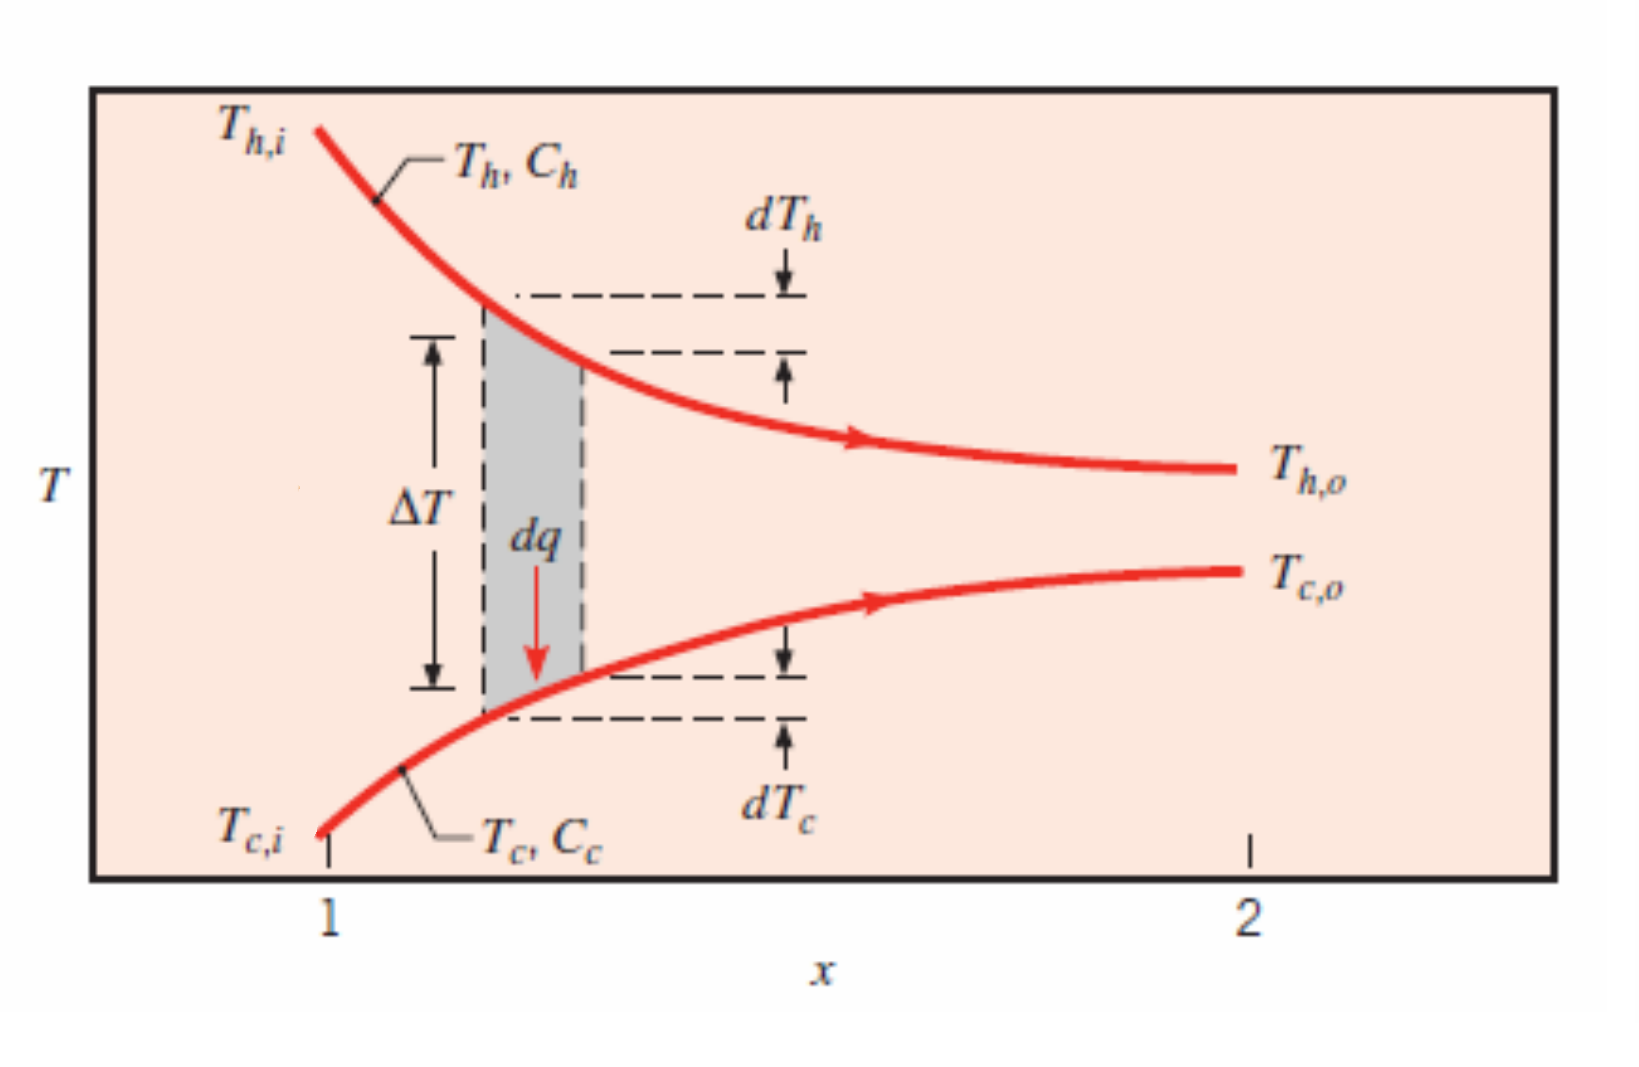
\includegraphics[width=0.45\textwidth]{parallele_flow_T}}\hfill
\subfloat[Temperature profil for counter flow HX \citep{Ngendakumana2018}\label{fig:C3_HX_opo_flow_T}] {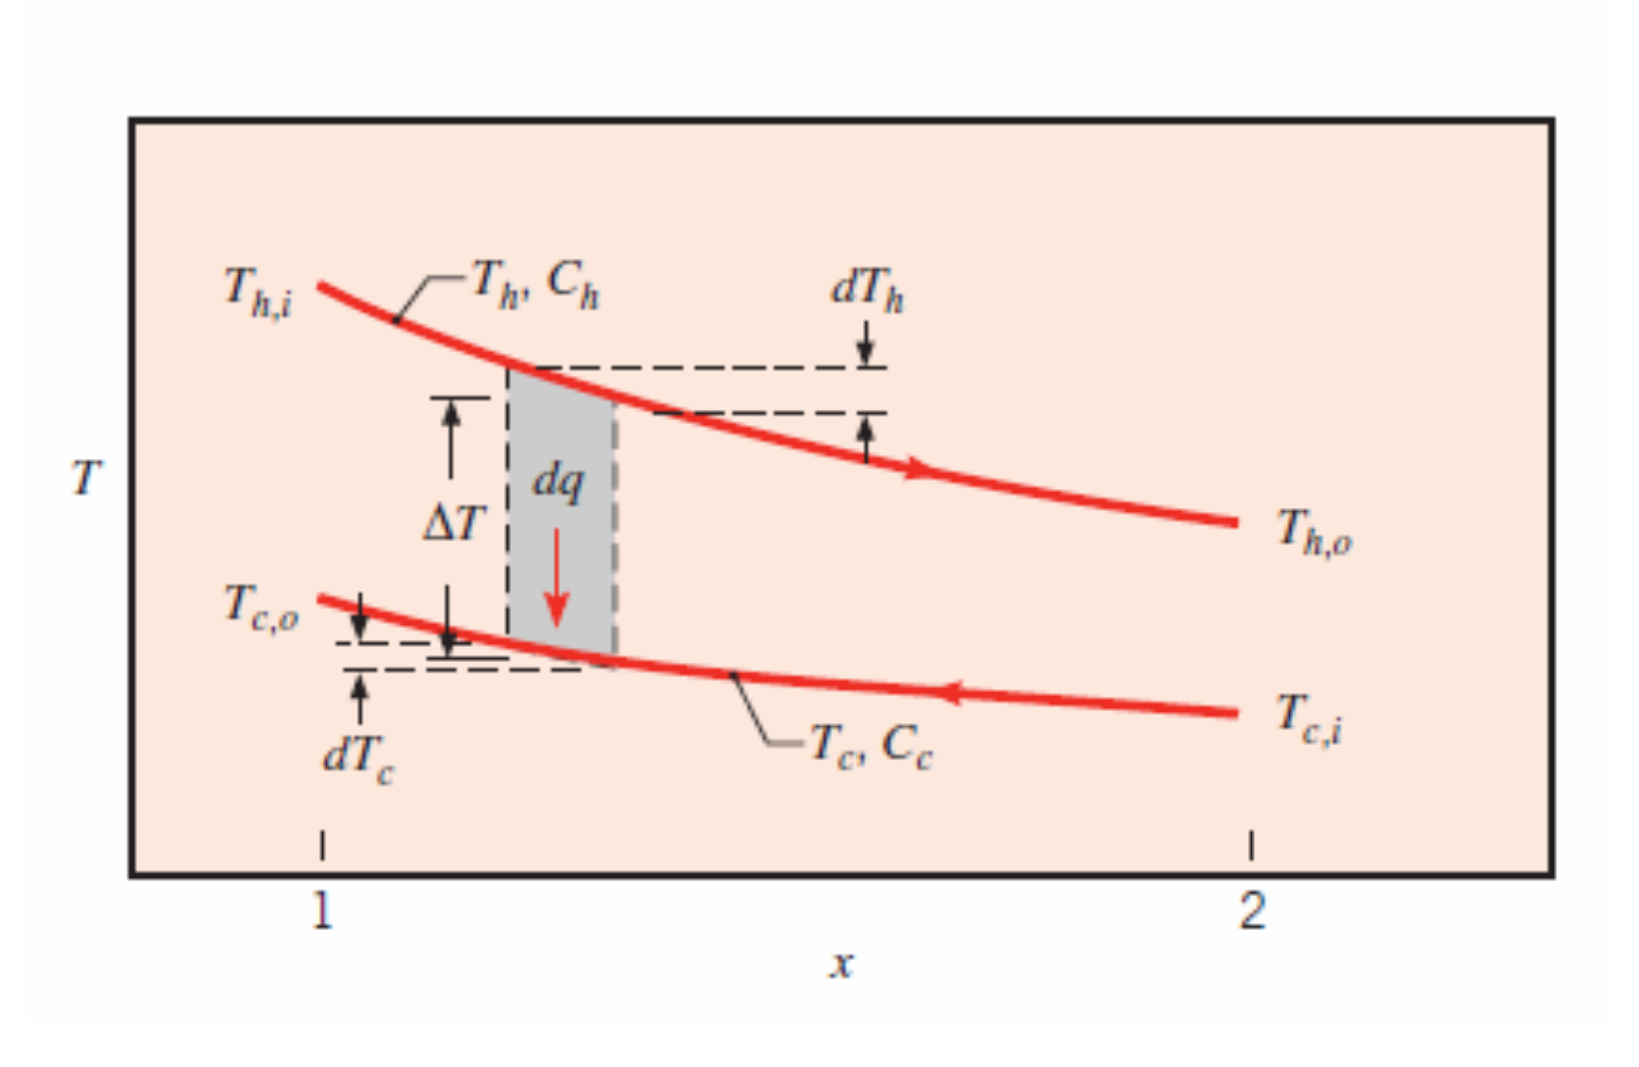
\includegraphics[width=0.45\textwidth]{opposite_flow_T}}\caption{Temperature profiles for different stream configurations}\label{fig:C3_Tprof}
\end{figure}

where the subscripts h and c indicate which flow is considered (h:hot; c:cold), and the subscripts i and o refer to the inlet and the outlet of the heat exchanger.

The first temperature difference $\Delta T_0$ is defined as being the largest temperature difference between the two flows, regardless the position inside the HX. Thus,

\begin{equation}
\setstretch{1}
\Delta T_0 =
\begin{cases}
T_{h,i} - T_{c,i} \text{ For the parallel flow}\\
T_{h,i} - T_{c,o} \text{ For the counter flow}\\
\end{cases}\label{eq:C3_DT0}
\end{equation}

The second temperature difference $\Delta T_L$ corresponds to the smallest temperature difference between the two flows. Thus,
\begin{equation}
\setstretch{1}
\Delta T_0 =
\begin{cases}
T_{h,o} - T_{c,o} \text{ For the parallel flow}\\
T_{h,o} - T_{c,i} \text{ For the counter flow}\\
\end{cases}\label{eq:C3_DTL}
\end{equation}

\subsection{Heat transfer within a heat-exchanger}
\quad\, The heat transfer rate of a heat exchanger is directly dependent on the nature of the fluids and the heat-exchanger itself. Let's consider the following relation (\ref{eq:C3_Qdot1})
\begin{equation}
\dot{Q} = \frac{\Delta T_{LM}}{R}= A\cdot U\cdot \Delta T_{LM}\text{ ( in W)}\label{eq:C3_Qdot1}
\end{equation}
where $A$ is the global surface area of the HX, and $R$ and $U$ are the global thermal resistance and transfer coefficient respectively. The $\Delta T_{LM}$ is called the logarithmic mean temperature difference. It's definition is
\begin{equation}
\Delta T_{LM} = \frac{\Delta T_0-\Delta T_L}{ln\left(\frac{\Delta T_0}{\Delta T_L}\right)}\label{eq:C3_lmtd}
\end{equation} 
with $ln$ being the neperian logarithm.
\subsubsection{Transfer coefficient}
The general definition for the product $A\cdot U$ is 
\begin{equation}
\frac{1}{A\cdot U}  = \frac{1}{\eta_{0,c}\cdot h_c \cdot A_c} + \frac{F_c}{\eta_{0,c}\cdot A_c} + R_w + \frac{F_h}{\eta_{0,h}\cdot A_h} + \frac{1}{\eta_{0,h}\cdot h_h \cdot A_h}\label{eq:C3_AU}
\end{equation}
where $h$ is the convective heat transfer coefficient (in W/m$^2$/K) of the fluid, $F$ is a degradation factor due to the clogging, $\eta_0$ is the global efficiency of the surface and $R_w$ is the wall resistance. 

It can be shown that the convective heat transfer coefficient $h$ is proportional to $\dot{m}^{4/5}$ for a turbulent stream in a smooth duct. Turbulent stream are stream for which the heat transfer coefficient is the much higher thanks to a large disorder within the flow. This type of flow is reached when the Reynolds number $Re$ exceeds a certain value. In circular tubes this critical value is around 10000.
\begin{align}
&Re = \frac{\rho\cdot v\cdot D_h}{\mu}\\
\text{ with $D_h = \frac{4\cdot A_c}{P_c}$}& \text{ and $u=\frac{\dot{m}}{\rho\cdot\pi\cdot\frac{D_h^2}{4}}$}
\end{align}
where $\mu$ is the static viscosity of the fluid, $A_c$ and $P_c$ are the area and the perimeter of the surface crossed by the flow, $D_h$ is the hydraulic diameter and $v$ is the velocity in the pipe.

In the present work, the heat exchanger that will be used are plate heat exchangers. For this specific category, the surface $A$ for the cold and the hot side are very closed from each others. Also, if the flow considered is only composed of one phase (i.e. only liquid or gaseous), the wall resistance $R_w$ can be neglected. 

If the efficiency $\eta$ are supposed equal for both the hot and the cold side and if the degradation factors $F$ are neglected, then the product $A\cdot U$ is proportional to
\begin{equation}
A\cdot U \div \frac{\dot{m}_h^{4/5}\cdot\dot{m}_c^{4/5}}{\dot{m}_h^{4/5} + \dot{m}_c^{4/5}}\label{eq:C3_AU_prop}
\end{equation}
\subsubsection{LMTD method}
\quad\, In the previous lines, a definition of the heat transfer rate based on the global transfer coefficient. This method is called the LMTD method and requires the knowledge of the geometry of the heat exchanger.
When the $\dot{Q}$ has been calculated, the temperatures at the outlet of the heat exchanger for the cold and hot stream can be computed using the two equations (\ref{eq:C3_ThQ}) and (\ref{eq:C3_TcQ}).
\begin{subequations}
\setstretch{1}
\begin{equation}
\dot{Q} = \dot{m}_h\cdot c_{p,h}\cdot(T_{h,in} - T_{h,out}) =\dot{C}_h\cdot(T_{h,in} - T_{h,out}) \label{eq:C3_ThQ}
\end{equation}
\begin{equation}
\dot{Q} = \dot{m}_c\cdot c_{p,c}\cdot (T_{c,out} - T_{c,in}) =\dot{C}_c\cdot (T_{c,out} - T_{c,in}) \label{eq:C3_TcQ} 
\end{equation}
\end{subequations}

This method requires the knowledge of the inlet and outlet temperatures of both fluids before initiating the computation of the heat transfer rate $\dot{Q}$ using the relation (\ref{eq:C3_Qdot1}). Therefore, this method needs iteration in the event where these temperatures are not known a priori.

\subsubsection{$\varepsilon$-NTU method}
\quad\, There exists a second method for the evaluation of the heat transfer rate which does not need the outlet temperature of the fluids. First, the maximum heat transfer rate $\dot{Q}_{max}$ is computed.
\begin{equation}
\dot{Q}_{max} = \dot{C}_{min}\cdot (T_{h,in} - T_{c,in})
\end{equation}
with $\dot{C}_{min}=min(\dot{C}_h,\dot{C}_c)$
Then the heat transfer rate is equal to 
\begin{equation}
\dot{Q} = \varepsilon\cdot\dot{Q}_{max}
\end{equation}
where $\varepsilon$ is the efficiency of the heat exchanger. This efficiency is a function of the ratio $C_r = \frac{\dot{C}_{min}}{\dot{C}_{max}}$, the flow arrangement, and the number of transfer unit NTU defined as being the ratio
\begin{equation}
\text{NTU} = \frac{A\cdot U}{\dot{C}_{min}}\label{eq:C3_NTU}
\end{equation}

As said, the relations $\varepsilon(\text{NTU},C_r)$ and $\text{NTU}(\varepsilon,C_r)$ depend on the heat exchanger configurations. An non exhaustive list is written in the annex \ref{annex_epsNTU}\citep{GregoryNellis2015} 
%%%%%%%%%%%%%%%
%ECRIRE ANNEXE%
%%%%%%%%%%%%%%%

Once the coefficient $\varepsilon$ computed, the outlet temperatures of the fluids can be obtained using the relations (\ref{eq:C3_ThQ}) and (\ref{eq:C3_TcQ}).

\subsubsection{Rating and sizing problem}
\quad\, The $\varepsilon$-NTU method is really useful for solving rating and sizing problems.

On one hand, rating problem are problem that, based on the knowledge of the geometry of the heat exchanger, evaluates its performance for given inlet temperature for both fluids. For this kind of problem, the NTU is first computed. Then, the efficiency $\varepsilon$ is derived to allow the calculation of the heat transfer rate.

On the other hand, sizing problems are used for the design of heat exchanger to provide the wished outlet temperatures. There, the efficiency is first calculated and then the NTU is deduced. Finally, from the equation (\ref{eq:C3_NTU}) the heat transfer area $A$ can be obtained\citep{Ngendakumana2018}.

A mix of these two types of problems will be used during this work. Indeed, the efficiency $\varepsilon$ of the heat exchangers in the system are known for a certain nominal flow rate.    The knowledge of the nominal efficiency provides the required tools to compute the product $A\cdot U_{nom}$ using the sizing problem methodology. 

Then, based on the approximation (\ref{eq:C3_AU_prop}), the $U$ for the given condition can be obtained since the heat transfer area $A$ remains unchanged. Finally, the non nominal $U$ can be used to compute the non nominal efficiency $\varepsilon$ using rating problem.